\documentclass{article}
\newtheorem{thm}{Theorem}
\setlength{\oddsidemargin}{0.25in}
\setlength{\textwidth}{6in}
\setlength{\topmargin}{-0.25in}
\setlength{\headheight}{0.3in}
\setlength{\headsep}{0.2in}
\setlength{\textheight}{9in}
\setlength{\footskip}{0.1in}
\usepackage{multirow}
\usepackage{fullpage}
\usepackage{graphicx}
\usepackage{amsthm}
\usepackage{amssymb}
\usepackage{url}
\usepackage{amsfonts}
\usepackage{algpseudocode}
\usepackage{mathtools}
\usepackage{listings}	
\newcommand{\quotes}[1]{``#1''}

\usepackage{hyperref}
\hypersetup{
    colorlinks=true,
    linkcolor=blue,
    filecolor=magenta,      
    urlcolor=blue,
}

\begin{document}\title{Homework 4\\ Introduction to Data Analysis and Mining \\ Spring 2018\\ CSCI-B 365}         % Enter your title between curly braces
\author{Instructor: Hasan Kurban}        % Enter your name between curly braces
\date{\today}          % Enter your date or \today between curly braces
\maketitle
\makeatother     % `@' is restored as a "non-letter" character
\pagestyle{plain}
\section*{Directions}
Please follow the syllabus guidelines in turning in your homework.  I am providing the \LaTeX{} of this document too. This homework is due Friday, March  16, 2018 10:00p.m. \textbf{OBSERVE THE  TIME}. Absolutely no homework will be accepted after that time. All the work should be your own.  
 
   %%%%%%%%%%%%%%%%%%%%%%%%%%%%%%%%%%%%%%
%                      PROBLEM 1
 %%%%%%%%%%%%%%%%%%%%%%%%%%%%%%%%%%%%%%


  \section*{Problem 1 [30 points]}  
  
In this question, you will first perform principal component analysis (PCA) over  \href{https://archive.ics.uci.edu/ml/datasets/ionosphere}{
Ionosphere Data Set} and then cluster the  reduced data using your $k$-means program ($C_k)$ from previous homework. You are allowed to use R packages for PCA and ignore the class variables (35th variable) while performing PCA. Answer the questions below:
 \\
  \begin{enumerate}
  \item[\textbf{1.1)}] Perform PCA over Ionosphere data set and make a scatter plot of PC1 and PC2 (the first two principal components). Are PC1 and PC2 linearly correlated?  
\\
\begin{lstlisting}
adata <- read.table("https://archive.ics.uci.edu/ml/machine-learning-databases/ionosphere/ionosphere.data", sep = ",")
inputdata <- subset(adata, select = -c(35))
pca2 = prcomp(inputdata)
plot(pca2$rotation, xlab = "PC1", ylab = "PC2")
\end{lstlisting} 	
\begin{figure}
  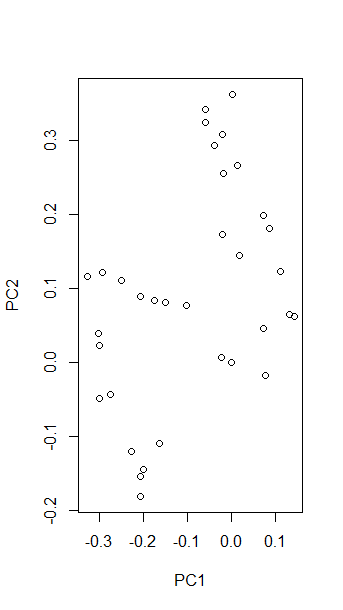
\includegraphics[width=100mm, scale = 0.5]{PC12.png}
  \caption{They are not linearly correlated}
\end{figure}
  \item[\textbf{1.2)}]  There are three methods to pick the set of principle components: (1) In the plot where the curve bends; (2)
Add the percentage variance until total $75\%$ is reached ($70-90\%$) (3) Use the components whose variance
is at least one. Show the components selected in the Ionosphere data  if each of these is used.
\\
\begin{lstlisting}
pca1 = PCA(inputdata, graph = FALSE)
pca2$rotation[order(pca2$rotation[,1]),1][pca2$rotation[order(pca2$rotation[,1]),1] >= -0.2 & pca2$rotation[order(pca2$rotation[,1]),1] <= 0] #where curve bends
pca1$eig[,3][pca1$eig[,3] <= 80]#keep variance at least 75
pca2$sdev[pca2$sdev^2 >= 1] #variance >= 1
\end{lstlisting}
  \item[\textbf{1.3)}]  Observe the loadings using prcomp() or princomp() functions in R and  discuss loadings in PCA?i.e., how are principal components and original variables related?
\\
\begin{lstlisting}
pca2$rotation
\end{lstlisting}
\paragraph{}
After observing the correlation between the variables and the factors. Almost all of the data has positive or negative correlation. Showing there is no correlation between each PC.
  \item[\textbf{1.4)}] Perform dimensionality reduction over Ionosphere data set with PCA.  Keep $90\%$ of variance  after PCA and reduce Ionosphere data set and call this data $\Delta_R$. Cluster  $\Delta_R$ using your $k$-means program from previous assignment and report the total error rates for $k = 2,\ldots,5$ for 20 runs each. Plots are generally a good way to convey complex ideas quickly, i.e., box plots, whisker plots. Discuss your results, i.e how did PCA affect  performance of $k$-means clustering.
\end{enumerate}  
\begin{lstlisting}
len = length(pca1$eig[,3][pca1$eig[,3] <= 90]) + 1
k1 = kmeans(pca1$eig[c(1:len),], 2, iter.max = 20, algorithm = "Lloyd", trace=FALSE)$tot.withinss
k2 = kmeans(pca1$eig[c(1:len),], 3, iter.max = 20, algorithm = "Lloyd", trace=FALSE)$tot.withinss
k3 = kmeans(pca1$eig[c(1:len),], 4, iter.max = 20, algorithm = "Lloyd", trace=FALSE)$tot.withinss
k4 = kmeans(pca1$eig[c(1:len),], 5, iter.max = 20, algorithm = "Lloyd", trace=FALSE)$tot.withinss
boxplot(k1,k2,k3,k4)
\end{lstlisting}
\begin{figure}
  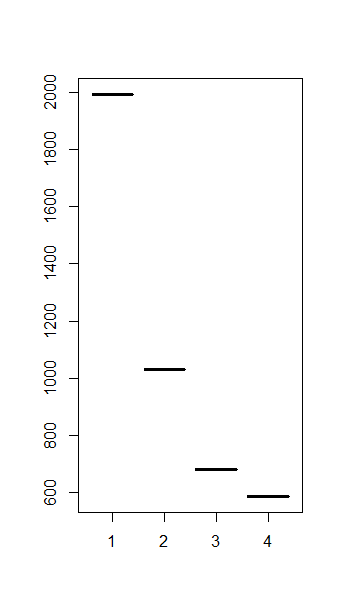
\includegraphics[width=100mm, scale = 0.5]{SSE.png}
  \caption{Total error rate decrease exponentially as k increase}
\end{figure}
\pagebreak
  %%%%%%%%%%%%%%%%%%%%%%%%%%%%%%%%%%%%%%
%                      PROBLEM 2
 %%%%%%%%%%%%%%%%%%%%%%%%%%%%%%%%%%%%%%
 \section*{Problem 2 [30 points]}  Randomly choose 50 points from Ionosphere data set (call this data set $\text{I}_{50}$) and perform hierarchical clustering. You are allowed to use R packages for this question. (Ignore the class variable while performing hierarchical clustering.)
 \\ 
 \begin{enumerate}
  \item[\textbf{2.1)}]  Using hierarchical clustering with complete linkage and Euclidean distance cluster $\text{I}_{50}$. Give the dendrogram.
\\ 
 \begin{lstlisting}
randomRows = function(df,n){
  return(df[sample(nrow(df),n),])
}
I50 = randomRows(inputdata, 50)
test = hclust(dist(I50))
plot(test)
\end{lstlisting}
\begin{figure}
  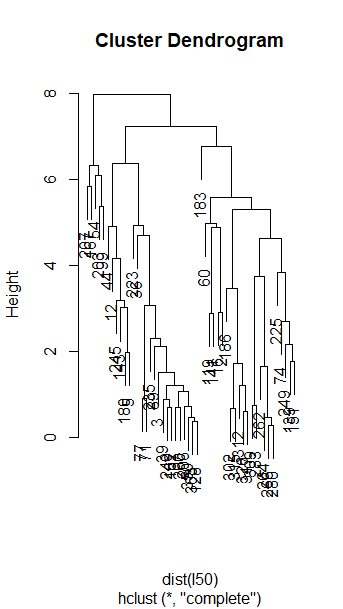
\includegraphics[width=100mm, scale = 0.5]{random.png}
\end{figure}
\item[\textbf{2.2)}] Cut the dendrogram at a height that results in two distinct  clusters. Calculate the error-rate.
\\  
 \begin{lstlisting}
cut1 = cutree(test, 2)
rate = errorRate(cut1,adata)
[1] 0.4219269
\end{lstlisting}

  \item[\textbf{2.3)}] First, perform PCA on $\text{I}_{50}$ (Keep $90\%$ of variance ). Then hierarchically cluster the reduced data using complete linkage and Euclidean distance. Report the dendrogram.
\\  
\begin{lstlisting}
pca3 = PCA(I50, graph = FALSE)
reduced = pca3$eig[,3][pca3$eig[,3] <= 90]
test2 = hclust(dist(reduced))
plot(test2)
\end{lstlisting}
\begin{figure}
  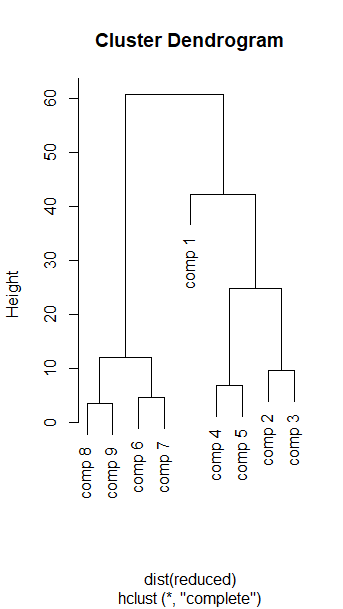
\includegraphics[width=100mm, scale = 0.5]{h2.png}
\end{figure}
    \item[\textbf{2.4)}]  Cut the dendrogram at a height that results in two distinct  clusters. Give the error-rate.  Discuss your findings, i.e., how  did PCA affect hierarchical clustering results?
\end{enumerate}
\begin{lstlisting}
cut2 = cutree(test3, 2)
rate2 = errorRate(cut2,adata)
[1] 1.1
\end{lstlisting}
\paragraph{}
After taking the PCA, the component used are significantly decrease, and making the dendrogram easily view. We also ignored some data by keeping a certain variance.
 %%%%%%%%%%%%%%%%%%%%%%%%%%%%%%%%%%%%%%
%                      PROBLEM 3
 %%%%%%%%%%%%%%%%%%%%%%%%%%%%%%%%%%%%%%
  \section*{Problem 3 [20 points]} 
From textbook, Chapter 8 exercises 16, 18 and 30 (Pages 563-566)
\begin{figure}
  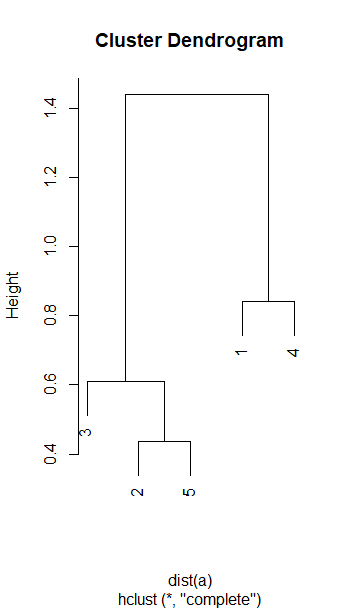
\includegraphics[width=100mm, scale = 0.5]{complete16.png}
  \caption{Question16 complete linkage}
\end{figure}
\begin{figure}
  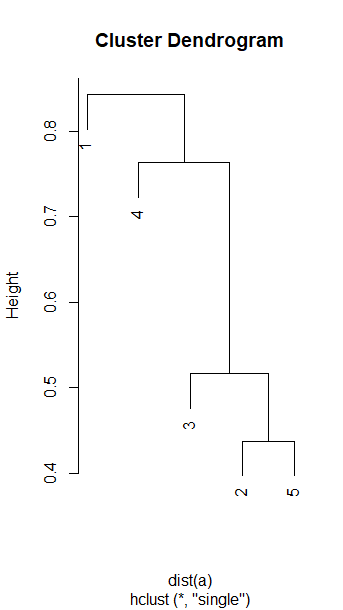
\includegraphics[width=100mm, scale = 0.5]{single16.png}
  \caption{Question16 single linkage}
\end{figure}
\paragraph{16}
Graphs are shown below. R code is provided in compressed file named "Q16.R"
\paragraph{18}
For both Ward's method and bisecting K-means have no refinement step.\\
Therefore, Ward's method, and besecting K-means represents a global minimum without removing unwanted elements. Ordinary K-means produces local minimum.
\paragraph{30a}
For the K means clustering of terms, it will cover all the terms, and the result will be not overlapping. However, the top terms clustering is likely to have many terms might not appear in the cluster as the threshold is specified.
\paragraph{30b}
Taking the top documents for the term cluster. 

 %%%%%%%%%%%%%%%%%%%%%%%%%%%%%%%%%%%%%%
%                   EXTRA CREDIT
 %%%%%%%%%%%%%%%%%%%%%%%%%%%%%%%%%%%%%%
  \section*{Extra Credit [10 points]} 

From textbook, Chapter 8 exercise 12 (Page 562).
\paragraph{12a}
The advantage of the leader algorithm is that it only needs one scan of the data, so this algorithm is more efficient.\\
The disadvantage is that leader algorithm cannot set the "k" cluster, and this algorithm tends to have worse sum of squared errors than the K-means algorithm.
\paragraph{12b}
Setting the cluster value in a different way that based on the distribution of the ordered data, as we can visualize the percentile on the box plot. Then we can assign data points to its according cluster. (i.e 25th percentile, 50th percentile, outliers etc.)\\


%%%%%%%%%%%%%%%%%%%%%%%%%%%%%%%%%%%%%%
\section*{What to Turn-in}
 Submit a .zip file that includes the files below. Name the .zip  file as \quotes{usename-section number}, i.e., hakurban-B365.


\begin{itemize}
\item The *tex and *pdf of the written answers to this document.
\item *\texttt{R}files for:
\begin{itemize}
\item R code for problem 1 (\quotes{pca1.R}).
\item R code for problem 2 (\quotes{hierarchical2.R}).
\end{itemize}
\end{itemize}




\end{document}


